\documentclass[a4paper,english,russian]{G2-105}
\usepackage[T1]{fontenc}
\usepackage{listings}
\usepackage{graphicx}
\usepackage{longtable}
\usepackage{booktabs}
\usepackage{standalone}
\usepackage{newclude}
\usepackage[final]{pdfpages}
\usepackage{multirow}
\usepackage{sansmath} % Enables turning on sans-serif math mode, and using other environments
\sansmath % Enable sans-serif math for rest of document
\usepackage[math]{blindtext}

%\usepackage[utf8]{luainputenc}
\VSTUSetDocumentNumbersPrefix{}
\VSTUSetDocumentCode{ВСТАВИТЬ КОД}
\VSTUSetDocumentTypeDative{выпускной работе бакалавра}
\VSTUSetDocumentTypeGenitive{выпускную работу бакалавра}
\VSTUSetInitialData{задание, выданное научным руководителем с кафедры САПР и ПК,
утвержденное приказом ректора}
\VSTUSetPZContents{
    \begin{VSTUList}
    \ulitem{Введение}
    \ulitem{1 Обзор используемых технологий}
    \ulitem{2 Описание математических моделей}
    \ulitem{3 Особенности программной реализации}
    \ulitem{4 Особенности тестового примера}
    \ulitem{5 Особенности архитектуры C.H.I.P.}
    \ulitem{6 Исследование скорости работы реализованного функционала}
    \ulitem{Выводы}
    \ulitem{Приложение A - Техническое задание}
    \end{VSTUList}
}
\VSTUSetPZGraphics{
    \begin{VSTUNumberedList}
    \ulitem{1: Название работы}
    \end{VSTUNumberedList}
}

\begin{document}
\VSTUSetOrder{????–ст}{??}{??????}{201?}
\VSTUSetFaculty{Электроники и вычислительной техники}
\VSTUSetDepartment{Системы автоматизированного проектирования и ПК}
\VSTUSetDepartmentCode{??.??}
\VSTUSetDirection{??.??.?? Автоматизированные системы управления}
\VSTUSetHeadOfDepartment{Зав. кафедрой САПР и ПК}{д.т.н., ??.}{М. В. Щербаков}{Щербаков Максим Владимирович}
\VSTUSetDirector{старший преподаватель САПР и ПК}{}{А. В. Катаев}{Катаев Александр Вадимович}
\VSTUSetFacilityExpert{}{}{}{}
\VSTUSetStandardsAdviser{????}{?????}{???????????}{?????? ?????? ????????????}
\VSTUSetStudent{ИВТ-461}{Т. А. Мельников}{Мельников Тимофей Алексеевич}
\VSTUSetTitle{Портирование сверточной нейросети на ARM архитектуру с ограниченными вычислительными ресурсами и ресурсами памяти}
\VSTUSetTitleEng{Porting a convolutional neural network on an ARM architecture, taking into account the computing resources and memory resources}
%\VSTUAddChapterWordToTOC % обязательно для ПЗ в магистерских диссертациях
\VSTUInitializePZ
\abstract{Аннотация}
\par Документ представляет собой пояснительную записку к выпускной работе бакалавра на тему «Портирование сверточной нейросети на ARM архитектуру с ограниченными вычислительными ресурсами и ресурсами памяти», выполненную студентом группы ИВТ-461, Мельниковым Тимофеем Алексеевичем.
\par В данной работе рассмотрена возможность реализации алгоритмов машинного обучения, в частности прямой проход сверточной нейронной сети, на устройстве с ограниченными вычислительными ресурсами и ресурсами памяти.
\par Объём пояснительной записки составил \totalpages~страниц и включает \totalfigures~рисунков и \totaltables~таблицы. 

%\newpage
\tableofcontents
\newpage

\starchapter{Введение}
\par Задачи обработки и анализа аналоговой информации являюся одини из самых сложных в IT-индустрии. Долгое
время такие задачи решались евристическими алгоритмами, которые требовали огромных аппаратных ресурсов при малой точности результата. С переоткрытием машинного обучения решения задач анализа изображений, аудиосигнала или текста поднялись на новый уровень. Алгоритмы машинного обучения позволяют находить неявные зависимости данных и строить адекватные модели.
\newpage

\chapter{Анализ состояния поддержки перечислений в типах вопросов системы дистанционного образования Moodle}
\ttl
\section{Обобщенное описание проблемы перечислений}

\par Основным достоинством формальных языков - жестко заданный порядок лексем в выражении. С другой стороны из жесткого порядка бывают исключения. Такие исключения чаще являются перечислениями, то есть последовательностью элементов отделенных разделителями друг от друга, порядок которых не важен.
\par Один из типичных примеров использования перечислений изображен на рисунке~\ref{question}.

\par Правильными ответами будут строки:
\begin{itemize}
    \item bool sign; unsigned int enom; unsigned int denom;
    \item bool sign; unsigned int denom; unsigned int enom;
    \item unsigned int enom; unsigned int denom; bool sign;
    \item unsigned int enom; bool sign; unsigned int denom;
    \item unsigned int denom; unsigned int enom; bool sign;
    \item unsigned int denom; bool sign; unsigned int enom;
\end{itemize}
\par Количество вариантов перестановок элементов в перечислении определяется, факториалом от числа его элементов. При наличии в ответе нескольких перечислений количество вариантов правильных ответов будет равно произведению чисел порядков каждого перечисления в отдельности.
\par При рассмотрении данного примера становиться ясно, что поддержка перечислений необходима.
\section{Обзор существующих решений}

\par Для осуществления анализа состояния поддержки перечислений, а так же обзора существующих решений, необходимо ввести термин перечисление. Перечислением называется последовательность элементов, состоящих из одной или нескольких лексем, порядок элементов в ответе не важен, они могут отделены друг от друга лексемами-разделителями.
\par На данный момент существует множество типов вопросов для СДО Moodle. Типы вопросов по разному отрабатывают ответы студентов, некоторые используют регулярные выражения, другие находят наибольшие общие части эталонного ответа и ответа данного студентом, третьи строят синтаксические деревья для поиска ошибок. В данной главе будут проанализированы основные плагины типов вопросов Pmatch, Preg и Correct Writing.

\subsection{Критерии анализа}

\par Главным требованием к разрабатываемой системе является интеграция с СДО Moodle. Данное требование было выдвинуто заказчиком, его актуальность объясняется использованием данной системы заказчиком.
\par Так же важным требованием является возможность внедрения поддержки перечислений в существующий модуль. Выбранные для анализа плагины, работают с ответом по разному, даже формат задания эталонного ответа различен. Из данного обстоятельства выплывает актуальность этого требования.
\par Довольно часто вопросы для тестов создаются обычными учителями, преподающих разные предметы, и имеющих различные уровни инженерного образования. Что требует возможности создания вопросов, а так же описаний перечислений в простой и понятной форме. То есть не требующих от учителя дополнительных познаний.
\par Таким образом, необходимо сравнить существующие системы по таким критериям, как возможность внедрения поддержки перечислений в существующий модуль, возможность интеграции в СДО Moodle, возможность создания вопросов и описаний перечислений в простой и понятной форме.  

\subsection{Тип вопроса PMatch}

\par Данный плагин разрабатывается сообществом Open University в рамках разработки СДО Moodle. Плагин позволяет проводить анализ ответа студента на основе шаблона заданного преподавателем. Шаблоны используемые плагином схожи с регулярными выражениями. Так же в плагине реализована проверка опечаток, проверка ответа с неполным совпадением.
\par В плагине присутствует частичная возможность описания перечислений с помощью альтернатив \cite{1}. Однако этот метод не лишен недостатков: 
\begin{itemize}
    \item при использовании альтернатив, есть возможность указать варианты лексем, для определенной позиции, но не возможно описать зависимости между лексемами. Что приводит к тому что при описании перечислений, будут порождаться неправильные ответы;
    \item так же при использовании шаблонов в связке с перечислениями, сложность описания правильного ответа будет возрастать, а уровень наглядности, будет уменьшаться.
\end{itemize}
\par Не смотря на то, что система не подходит для решения поставленной задачи, так как в ней не возможно реализовать описание и обработка перечислений, она подходит для решения других задач. В частности, на текущий момент, данная система используется для обучения различным предметам и обработки результата ответа на естественном языке, где перечисления отсутствуют. 

\subsection{Тип вопроса Preg}

\par Данный плагин разрабатывается на кафедре "Программное обеспечение автоматизированных систем"\ Волгоградского государственного технического университета,  под руководством к.т.н. Сычева О.А. Плагин производит анализ ответа студента на основе заданного преподавателем регулярного выражения. Так же плагин позволяет выводить подсказки о следующем символе, лексеме. Так же преподавателю предоставлена возможность просмотра графа построенного на основе заданного выражения, его синтаксического дерева и словесного описания. Более того есть возможность проверки регулярного выражения вводом примеров ответов \cite{2}. 
\par В плагине присутствует возможность описания перечислений на основе использования альтернатив. Регулярные выражения во многом схожи с шаблонами, но имеют под собой четкую и проработанную математическую базу. Данный подход имеет общие недостатки с шаблонным подходом. Кроме этого данный плагин сложнее в использовании и понимании, так как вопросы строятся с использованием математической системы и представления ответа в виде графа. То есть плагин требует специфических знаний. 
\par Так же как и в предыдущей системе подход к обработке перечислений изменить невозможно. Следовательно система не подходит для решения данной задачи.

\subsection{Тип вопроса Correct Writing}

\par Плагин Correct Writing также является разработкой кафедры "Программное обеспечение автоматизированных систем" Волгоградского государственного технического университета, под руководством Сычева О.А. Плагин основан на синтаксическом анализе ответов преподавателя и студента. Плагин позволяет выделять лексические и синтаксические ошибки студента. А также демонстрировать объяснение ошибки студенту в двух вариантах: в формате текстового сообщения или графического изображения \cite{3,4}.
\par Плагин не позволяет описывать перечисления. Единственный способ описать ответ содержащий перечисления - это полный перебор порядков элементов перечисления, что влечет за собой необходимость ввода описаний каждой лексемы для каждого варианта эталонного ответа.
\par Однако с другой стороны, данный плагин не использует специфических описаний, эталонный ответ, записывается как есть. Что позволяет говорить о том, что данный плагин прост и понятен для преподавателей, вне зависимости от предмета который они преподают и специфики их знаний. 
\par Еще одним положительным моментом является возможность внедрения в плагин поддержки перечислений.

\section{Анализ полученных результатов}
\par Перед тем, как проводить анализ полученных результатов при помощи метода анализа иерархий,  проведем первичный анализ результатов.
\par Все анализируемые системы (PMatch, Preg, CorrectWriting) являются плагинами для СДО Moodle, следовательно, из процесса сравнения данный критерий исключается как выполняющийся для всех систем.
\par Сформируем матрицу весов критериев. Для этого, проранжируем данные критерии по важности.
\par В процессе анализа было выявлено два критерия – возможность внедрения перечислений, возможность создания вопроса в простой и понятной форме. Определим их относительную важность.  Первый критерий имеет существенную значимость над вторым. Исходя из ранжирования критериев Саати \cite{5},  можно составить матрицу, строками которой будут последовательности (1, 6), (0.165, 1). Вычисляя собственные значения данной матрицы, мы получим значения весов равные 2.45,  0.408. Нормализуя данный вектор, получаем значения весов  равные  0.857, 0.143. 
\par Проранжируем значения критериев. Для всех критериев возможно установить два значения – отсутствует, с численным значением «0», и присутствует,  с численным значением «1».
\par Из таблицы 1 видно, что наилучшим вариантом является CorrectWriting. Так как удовлетворяет приведенным критериям.
\par Другие варианты, такие Preg, а также PMatch, нельзя признать до конца применимыми к данной задаче, так как они не обеспечивают возможности внедрения поддержки перечислений. 
\\ \\ \ttl \ttl \ttl\vspace*{14pt}
\begin{longtable}{|c|c|c|c|c|}
    \caption{Результаты анализа систем}\\ \hline
    \multirow{4}{*}{Системы} & Внедрение & Простота & Общая & Нормализованная \\ 
                                    & перечислений & создания & оценка & оценка \\ 
                                    &   & вопроса & &  \\ \cline{2-5} 
                                    & 0.857 & 0.143 & &\\ \hline \endhead
    PMatch & 0 & 0 & 0 & 0 \\ \hline
    Preg & 0 & 1 & 0.143 & 0.125 \\ \hline
    CorrectWriting & 1 & 1 & 1.0 & 0.875 \\  
\end{longtable}

\starsection{Цель и задачи исследования}
\par Целью данной работы является снижение трудоемкости создания вопросов типа Correct Writing для изучения формализованных языков, с помощью поддержки перечислений.
\par Для достижения поставленной раннее цели необходимо решить следующие задачи:
\begin{itemize}
    \item исследовать спецификации языков C/C++, выбрать структуры языка, которые могут быть записаны в любом порядке, не изменяя работы программы;
    \item разработать алгоритм определения наилучшего порядка элементов перечисления;
    \item реализовать разработанный алгоритм и оценить качество его работы;
    \item интегрировать алгоритм в структуру плагина Correct Writing.
\end{itemize}
\par Исходя из этого, в первую очередь, необходимо выбрать те операторы языка, которые позволяют включать в себя перечисления. 

\chapter{Разработка модуля поддержки перечислений}
\ttl
\section{Описание интеграционных особенностей модуля}

\par Структуру модуля CorrectWritting наиболее точно отражает диаграмма компонентов, изображенная на рисунке ~\ref{component} \cite{6}.
\begin{figure}
    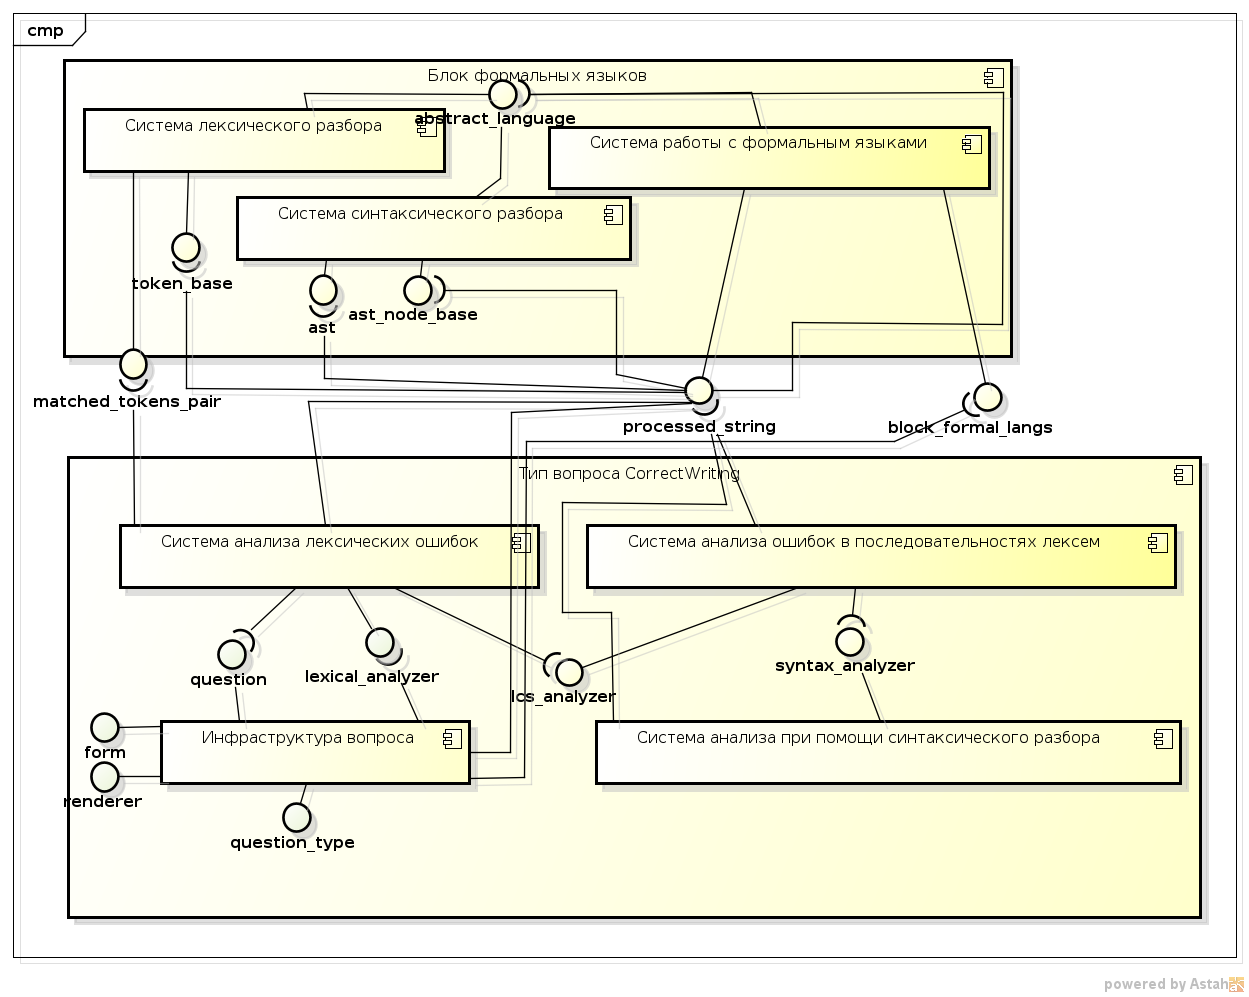
\includegraphics[width=\linewidth]{component.png}
    \caption{Диаграмма компонентов модуля CorrectWriting}
	\label{component}
\end{figure}
\par Процесс обработки ответа студента представлен на диаграмме потоков, рисунок ~\ref{dfd} \cite{7}.
\newpage
\begin{figure}
    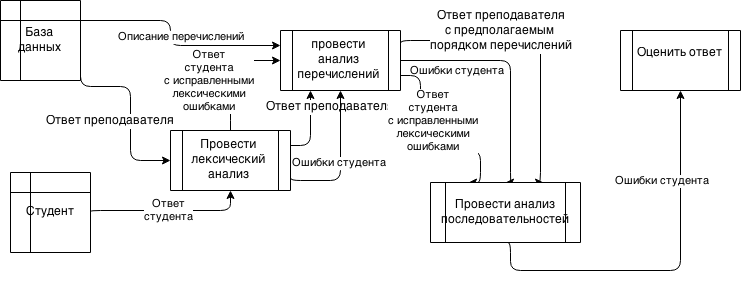
\includegraphics[width=\linewidth]{dfd1.png}
    \caption{Диаграмма потоков данных модуля CorrectWriting}
	\label{dfd}
\end{figure}
\par Для каждого этапа анализа ответа, реализован собственный анализатор. Все анализаторы используют один и тот же набор входных и выходных данных. Набор входных данных представляет собой совокупность эталонного ответа, ответа студента, а также вектор найденных ранее ошибок. А набор выходных совокупность ошибок, найденных на этапе анализа, и в некоторых случаях исправленный ответ студента. 
\par Исходя из структуры модуля было принято решение, разработать дополнительный анализатор определяющий  порядок лексем в эталонном ответе, который позволяет получить наибольшую общую подпоследовательность двух ответов студента и эталонного. Дополнительным  входным параметром будет описание перечислений соответствующие эталонному ответу. 
С другой стороны необходимо разработать средство для ввода описаний перечислений при создании нового вопроса. С этой целью было принято решение разработать модуль, определяющий возможные перечисления в эталонном ответе для языков C\textbackslash C++, а также графический модуль позволяющий исправить найденные ранее описания, а также добавить новые, в специфических случаях, а также в случае создания вопроса с ответом на других языках.

\section{Разработка модели представления перечислений}
\par Описанием перечислений является вектор описаний элементов перечислений. Описанием элемента перечисления есть вектор двух чисел - номеров первой и последней лексем принадлежащих элементу.
\par После определения порядка внедрения, в существующую систему, встает вопрос о том какие данные необходимо хранить для работы модуля, а также вопрос о формате их хранения.
\par Так как в модуле, каждый из анализаторов, является отключаемым, необходимо разработать формат позволяющий обеспечить безаварийную работу, в случае отключения разрабатываемого модуля. 
\par Наиболее точно описать перечисления можно описав границы его элементов. Описанием элемента перечислений служит пара индексов первой и последней лексем принадлежащих элементу в эталонном ответе. Тогда вектор описаний элементов перечислений, будет служить его описанием.
\par В CorrectWriting используется специфический класс связывающий пару ответов, эталонный и студента. Так как анализатор перечислений изменяет копию правильного ответа, было принято решение расширить класс эталонным ответом с измененным порядком лексем.
\par Так же существует проблема вложенности перечислений. Суть ее заключается в том, что при наличии вложенных перечислений, при перестановке элементов перечисления-контейнера, описания вложенного перечисления необходимо обновлять.
\section{Исследование стандартов языка С\textbackslash C++}
\par Для разработки модуля определения перечислений для языков C\textbackslash C++, необходимо выделить правила выделения перечислений. С целью выделения таких правил было проведено исследование стандартов языка C\textbackslash C++ \cite{8,9}. 
\par В ходе анализа были выделены правила описанные в таблице ~\ref{rules}:
\begin{longtable}{|c|l|}
    \caption{Результаты исследования стандартов языка C\textbackslash C++}  \label{rules} \\ \hline
    Операция & Правило \\ \hline 
    \endfirsthead
    \hline
    Операция & Правило \\ \hline 
    \endhead
    Сложение          & Оба аргумента данной операции являются \\ \cline{1-1}
    Умножение         & являются элементами перечисления. \\ \cline{1-1}
    Конъюнкция        & В случае нескольких подряд идущих \\ \cline{1-1}
    Дизъюнкция        & операций одного типа, все их  аргументы\\ \cline{1-1}
    Эквивалентность   & являются элементами перечисления.\\ \cline{1-1}
    Не эквивалентность& \\  \cline{1-1} 
    Битовое "И"       & \\  \cline{1-1}
    Битовое "ИЛИ"     & \\  \cline{1-1}
    Битовое           & \\
    исключающее "ИЛИ" & \\ \hline

    Деление           & Для нескольких подряд идущих операций \\ \cline{1-1}
    Вычитание         & одного типа, все их аргументы, \\ \cline{1-1}
    Целочисленное     & кроме первого, являются элементами \\  
    деление           & перечисления.\\ \hline
    Присваивание      & Для нескольких подряд идущих операций \\
                      & присваивания, все их аргументы, кроме \\
                      & последнего, становятся элементами \\
                      & перечисления.  \\ \hline
    Объявление        & Все объявленные перечислители являются \\
    перечисляемого    & элементами перечисления. \\  
    типа              & \\ \hline 
    Объявление        & Все объявленные переменные, в том числе \\
    переменных        & указатели, включая инициализацию, \\
    одного типа       & при ее наличии, являются элементами \\
                      & перечисления. \\  \hline 
    Объявление        & Все уровни доступа и слоты являются \\
    классов           & элементами перечисления. Все \\ 
                      & поля, прототипы функций, функции с \\
                      & реализацией одного уровня доступа \\
                      & являются элементами перечисления. \\ \hline 
    Объявление        & Все объявленные поля структур \\
    структур         & являются элементами перечисления.\\  \cline{1-1}
    Объявление        & \\
    объединений       & \\   
\end{longtable}
\par Для определения перечислений в сложных случаях, когда автоматически это сделать не удается, таких как объявление переменных разных типов, объявления с присваиванием объявленной ранее переменной, было принято решение разработать графический интерфейс редактирование перечислений. Требования к графическому интерфейсу, а также макеты представлены в приложении А. 
\section{Разработка алгоритмов решения задач}

\par Для решения задачи обработки перечислений был разработан следующий алгоритм работы модуля:
\begin{enumerate}
    \item проверка входных данных, то есть описания перечислений;
    \item поиск порядка изменения перечислений с учетом вложенности;
    \item поиск возможных порядков перечислений;
    \item выбор наиболее подходящих порядков.
\end{enumerate}

\subsection{Алгоритм проверки входных данных}

\par Для разработки данного алгоритма, для начала необходимо определить критерии оценки корректности входных данных. Так как входными данными является описание перечислений в эталонном ответе, необходимо определить критерии корректности описаний. Этими критериями являются:
\begin{itemize}
    \item отсутствие пересечений элементов перечислений;
    \item вложенность перечислений разрешена, но при условии что вложенное перечисление вложено только в один элемент другого или является разделителем только двух элементов;
    \item элементы перечислений не выходят за границы предложения.
\end{itemize}
\par Исходя из выше сказанного, алгоритм проверки входных данных, описывается следующей последовательностью шагов:
\begin{enumerate}
    \item проверить отсутствие пересечений элементов, внутри перечислений, и между перечислениями;
    \item проверить правильность вложенности перечислений;
    \item проверить, не выходят ли перечисления за границы предложения.
\end{enumerate}
\par Входными данными к данному алгоритму являются описания перечислений в эталонном ответе.

\subsection{Алгоритм поиска порядка изменения перечислений с учетом вложенности}

\par Необходимость данного алгоритма, объясняется тем, что при наличии вложенности, перестановки одного перечисления, влияют на позиции элементов другого. Из этого следует необходимость задания строгой очереди изменения порядков элементов перечислений. При этом вложенные перечисления необходимо обработать, раньше перечислений-хранилищ. Вложенность одного перечисления в другое можно определить из их описаний, по следующим правилам:
\begin{itemize}
    \item если все элементы перечисления включены в границы одного элемента другого перечисления, то это перечисление вложено;
    \item если все элементы перечисления заключены между границами элементов другого, то это перечисление вложено;
\end{itemize}

\par Алгоритм поиска порядка изменения перечислений с учетом вложенности, в соответствии с определенными выше правилами, описан на рисунке ~\ref{apvp}.

\begin{figure}
    \center 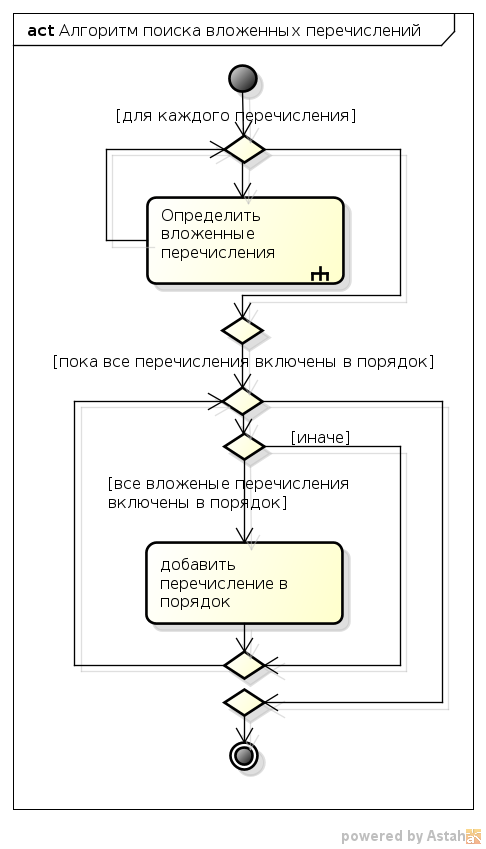
\includegraphics[height = 0.5\paperheight]{apvp.png}
    \caption{Алгоритм поиска порядка изменения перечислений с учетом вложенности}
	\label{apvp}
\end{figure}
\par Входными данными к данному алгоритму являются описания перечислений в эталонном ответе.

\subsection{Алгоритм поиска возможных порядков}

\par Данный алгоритм используется для исключения полного перебора вариантов правильного ответа. Этот алгоритм сводиться к полному перебору только в двух ситуациях:
\begin{itemize}
    \item если в предложении отсутствуют элементы перечислений;
    \item если в предложении для каждого перечисления элементы перечислений или отдельные лексемы им принадлежащие записаны в последовательности из которой можно получить все возможные порядки элементов перечисления. 
\end{itemize}
\par Алгоритм поиска возможных порядков, описан на рисунке ~\ref{apvp1}.
\begin{figure}
    \center 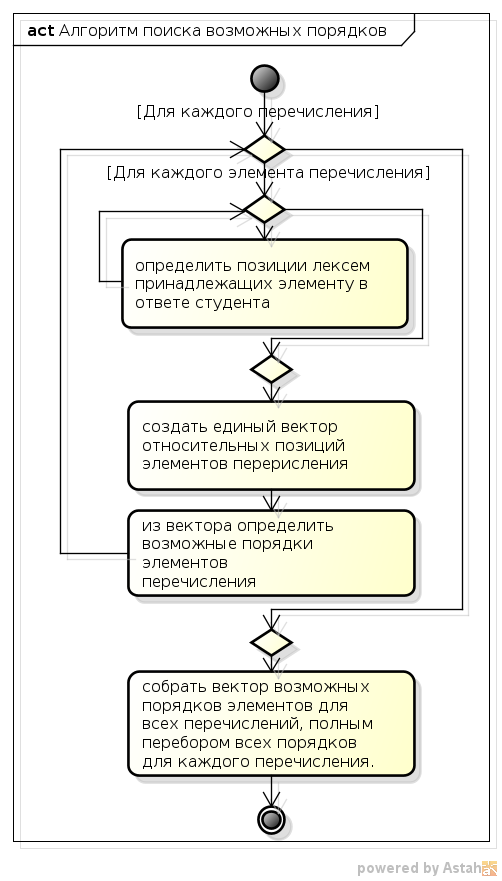
\includegraphics[height = 0.5\paperheight]{apvp1.png}
    \caption{Алгоритм поиска возможных порядков}
	\label{apvp1}
\end{figure}
\newpage
\par Входными данными к данному алгоритму являются описания перечислений в эталонном ответе, эталонный ответ, ответ студента.

\subsection{Алгоритм выбора наиболее подходящих порядков}

\par Во-первых необходимо определить критерий выбора наиболее подходящих порядков. Так как мы сравниваем два ответа между собой, этим критерием является наибольшая общая часть двух ответов. Следовательно наиболее подходящие порядки, будут те порядки, использование которых порождает наибольшую общую часть двух ответов.
\par Алгоритм выбора наиболее подходящих порядков, описан на рисунке ~\ref{avnpp}.
\newpage
\begin{figure}
    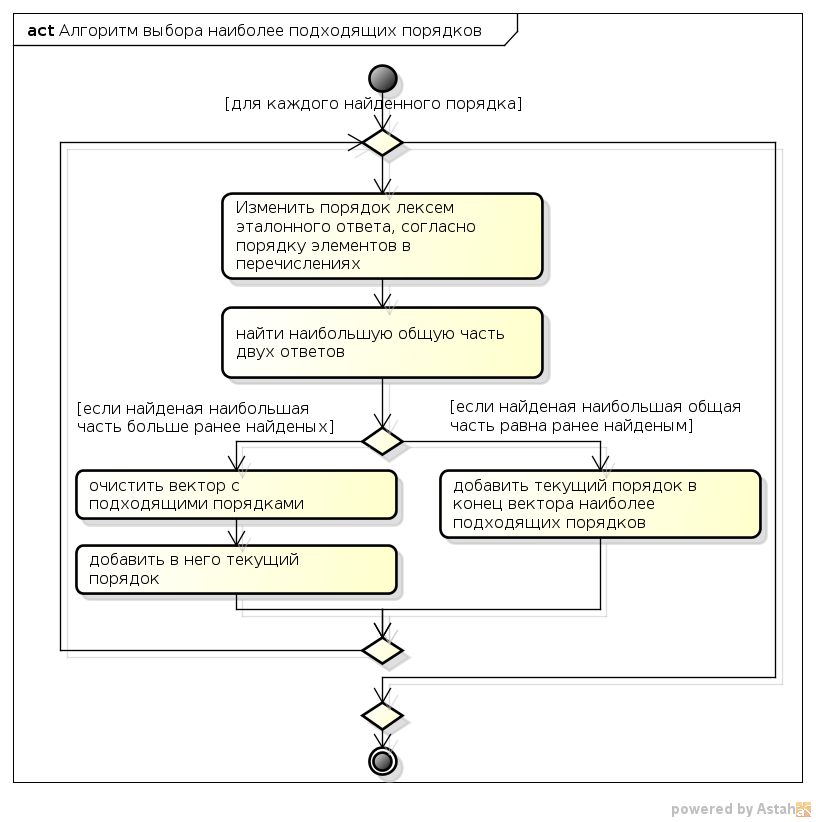
\includegraphics[height = 0.5\paperheight ,width=\linewidth]{avnpp.png}
    \caption{Алгоритм выбора наиболее подходящих порядков}
	\label{avnpp}
\end{figure}
\par Входными данными к данному алгоритму являются описания перечислений в эталонном ответе, эталонный ответ, ответ студента.

\section{Оценка принятого решения}

\par Данный алгоритм сложнее использования полного перебора, сложность которого описана в формуле (1).
\\ \hfill \\
\hspace*{66mm}    O(N*M*K),  \hspace*{62mm} (1) \\
\hfill \\ 
где N - число вариантов правильных ответов; \\
\hspace*{8 mm}M - число лексем правильного ответа; \\
\hspace*{8 mm}K - число лексем в ответе студента. 
\par Приведенный алгоритм имеет сложность описанную в форуле (2). \\ 
\hfill \\
\hspace*{51mm} O(R*M*K*Z*X$^2$*Y*E*P), \hspace*{44mm}(2) \\
\hfill \\
где R - количество найденных вариантов правильного ответа 1 $\leq$ R $\leq$  N, \\
\hspace*{8 mm}Z - число лексем принадлежащих перечислениям в правильном ответе;\\
\hspace*{8 mm}Y - число элементов в перечислении;\\
\hspace*{8 mm}X - число перечислений; \\
\hspace*{8 mm}E - число лексем элемента перечисления найденных в ответе студента; \\
\hspace*{8 mm}P - число найденных порядков элементов перечисления.
\par С другой стороны, несмотря на возросшую сложность, алгоритм работает быстрее полного перебора, из-за более простых внутренних операций над ответами.
\par Еще одним плюсом данного решения является уменьшения трудоемкости создания новых вопросов. Это объясняется отказа от необходимости полного перебора, в пользу добавления описания перечисления для одного правильного ответа.

\starsection{Выводы}

\par Введение специального алгоритма позволит отказаться от полного перебора вариантов, за исключением сложных случаев, когда в ответе студента содержаться все варианты перестановки элементов для каждого перечисления. Так же процесс создания нового вопроса становиться прост и понятен. 

\chapter{Оценка разработанного решения}
\ttl
\section{Описание процесса интеграции}
\par Интеграция в модуль происходила в двух направлениях:
\begin{itemize}
    \item интеграция в процесс создания ответа;
    \item интеграция в процесс оценивания ответа.
\end{itemize}
\par Интеграция в процесс создания ответа, заключается в добавлении к форме создания и редактирования вопроса окна редактирования перечислений для каждого эталонного ответа.
А также реализации сериализации и десериализации описаний перечислений, для хранения в базе данных.
\par Интеграция в процесс оценивания ответа, заключается во включении в процесс нового анализатора, и реализации адекватного взаимодействия анализаторов.
\section{Оценка структурной целостности решения}
\par Модуль разрабатывался с использованием объектно-ориентированного подхода \cite{10,11}. 
\par Модуль соответствует требуемому сообществом разработчиков Moodle стилю написания кода для языков PHP и JavaScript \cite{12,13,14}.
\par Часть модуля связанная с работой на клиенте, написана с использованием библиотеки Yui \cite{15}, являющийся официальной библиотекой используемой в Moodle.
\par На рисунке~\ref{class}, прадставлен фрагмент диаграммы классов типа вопроса CorrectWriting. 
\newpage
\begin{figure}
    \center 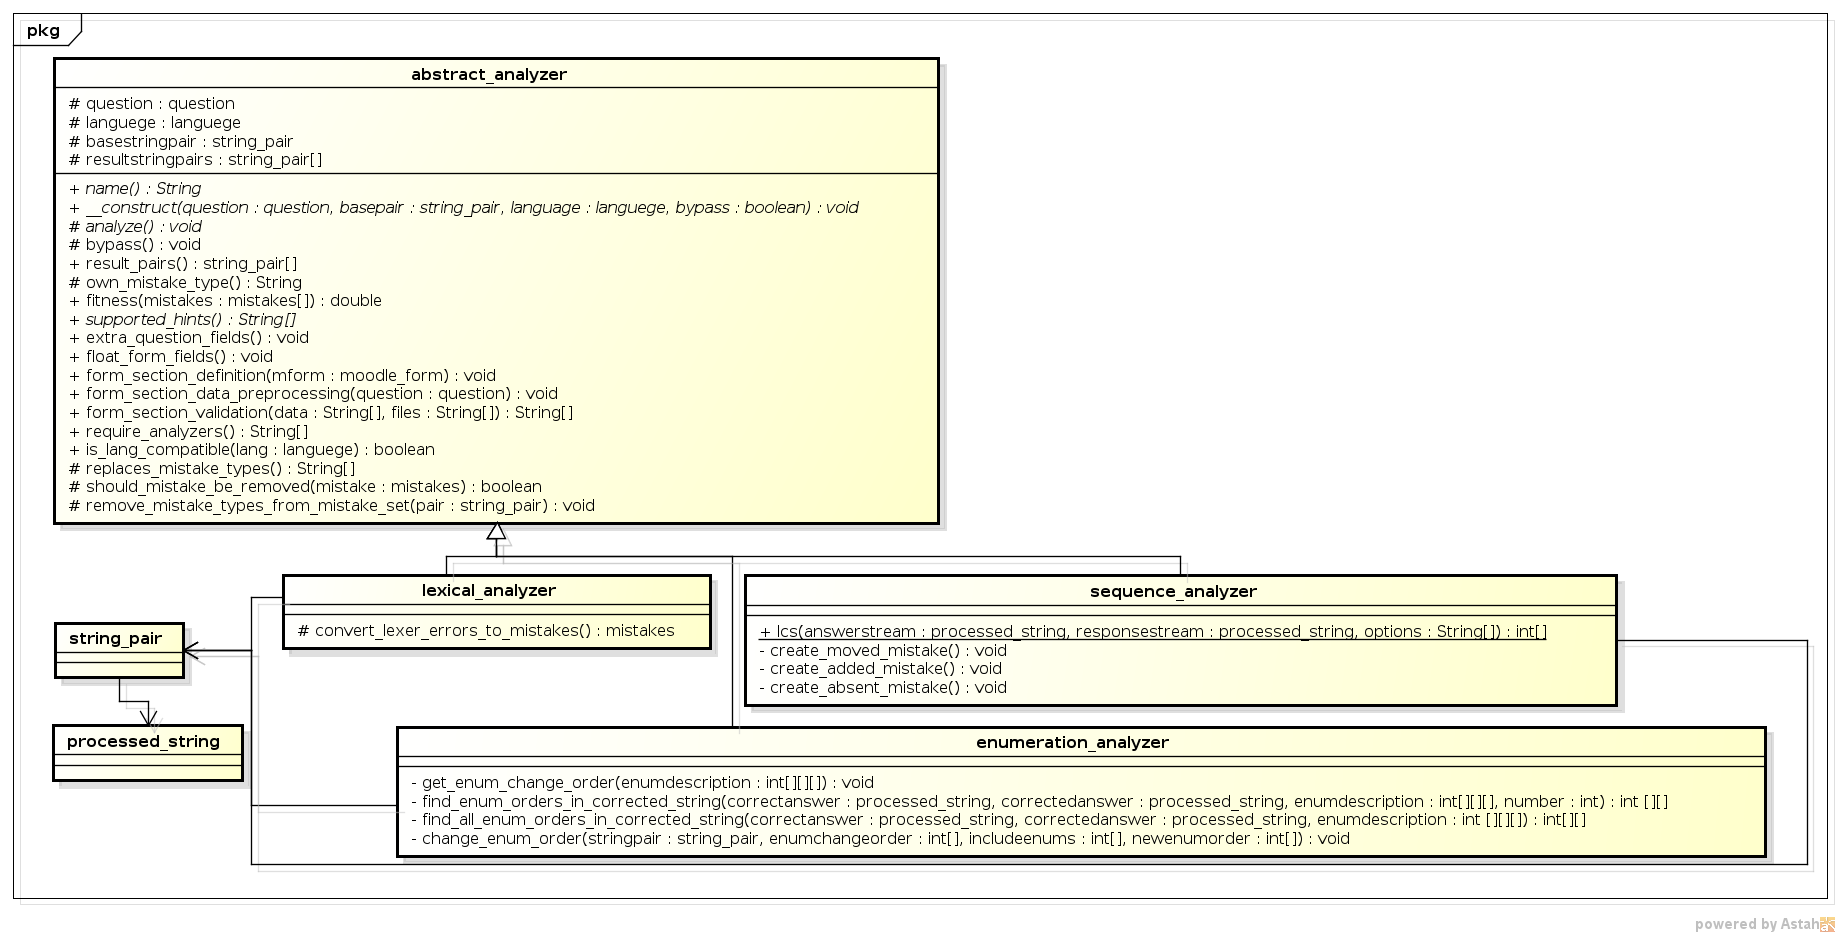
\includegraphics[width = \linewidth]{class.png}
    \caption{Фрагмент диаграммы классов}
	\label{class}
\end{figure}
\par Enumeration analyzer разработан как часть модуля. Его методы являются реализаций алгоритмов описанных во второй части данной пояснительной записки. Соответствие алгоритмов методом представлено в таблице ~\ref{am}.
\\ \\ \ttl \ttl \ttl\vspace*{14pt}
\begin{longtable}{|c|c|}
    \caption{Соответствие методов алгоритмам }\\ \hline
    \label{am} 
    Алгоритм & Метод \\ \hline \endhead
    алгоритм поиска порядка & get\_enum\_change\_order\\
    изменения перечислений с учетом & \\ 
    вложенности &  \\ \hline
    алгоритм поиска возможных &find\_enum\_orders\_in\_corrected\_ \\
    порядков & string и\\
             & find\_all\_enum\_orders\_in\_corrected\_ \\
             & string\\ \hline
    алгоритм выбора наиболее & change\_enum\_order и \\
    подходящих порядков & analyze\\
\end{longtable}
\par Метод find\_enum\_orders\_in\_corrected\_string находит предполагаемые порядки перечисления в ответе студента.
\par Метод find\_all\_enum\_orders\_in\_corrected\_string, используя find\_enum\_orders\_in\_corrected\_string, находит порядки для всех перечислений и создает варианты порядка лексем для эталонного ответа.
\par Метод change\_enum\_order изменяет порядок лексем в эталонном ответе, а также обновляет описание перечислений.
\par Метод analyze является главным в модуле. Он объединяет работу всех модулей, и выбирает наиболее подходящие эталонные ответы.
\par На диаграмме последовательности, представленной на рисунке ~\ref{sequence}, описан процесс интеграции в процесс оценивания ответа студента.
\begin{figure}
    \center 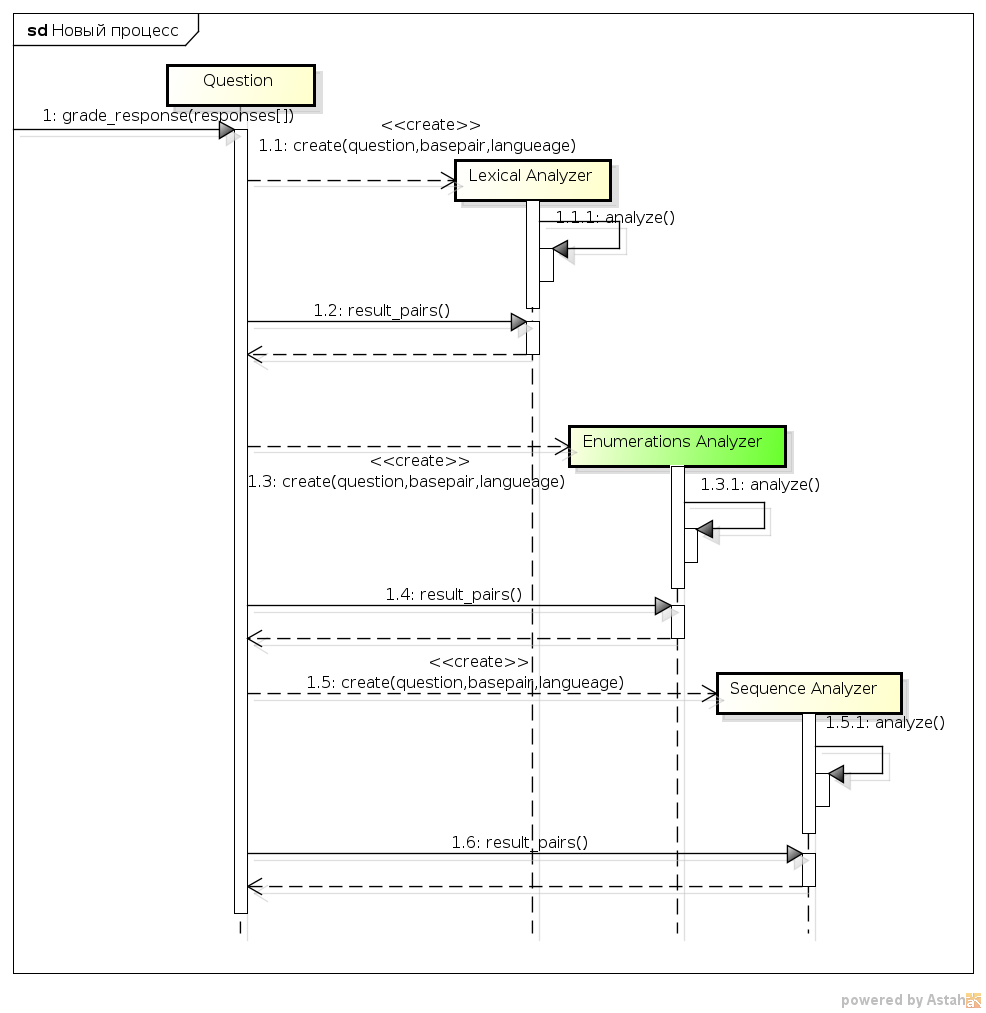
\includegraphics[width = \linewidth]{tzsequence.png}
    \caption{Диаграмма последовательности}
	\label{sequence}
\end{figure}

\section{Оценка работы модуля на тестовом примере}
\par Тестирование проведено на трех примерах:
\begin{enumerate}
    \item тестирование работы графического интерфейса в \\ приложении А;
    \item тестирование работы анализатора на этапе оценивания ответа в приложении А;
    \item тестирование скорости работы серверной части, по сравнению с CorrectWriting без разработанного модуля.
\end{enumerate}
\par Модуль выдержал тестирование графического интерфейса и тестирование работы анализатора на этапе оценивания ответа. 
\par Так же были разработаны модульные тесты:
\begin{enumerate}
    \item для анализатора перечислений 36 тестов, на работу всех функций модуля;
    \item для определения перечислений 29 тестов, на все правила;
    \item интеграционное тестирование 15 тестов, на взаимодействие всех анализаторов.
\end{enumerate} 
\par Тестирование скорости работы серверной части, будет рассмотрено подробнее. В качестве эталонного ответа используется строка "t == a || b \&\& c || k != true;", содержащая четыре перечисления:
\begin{enumerate}
    \item перечисление связанное с эквивалентностью, элементами которого являются: 
        \begin{enumerate}
            \item лексема "t";
            \item лексема "a";
        \end{enumerate}
    \item перечисление связанное с логическим сложением, элементами которого являются:
        \begin{enumerate}
            \item лексема "b";
            \item лексема "c";
        
        \end{enumerate}
    \item перечисление связанное с не эквивалентностью, элементами которого являются: 
        \begin{enumerate}
            \item лексема "k";
            \item лексема "true";
        \end{enumerate}
    \item перечисление связанное с логическим умножением, элементами которого являются:
        \begin{enumerate}
            \item перечисление связанное с эквивалентностью, то есть подстрока "t == a";
            \item перечисление связанное с логическим сложением, то есть подстрока "b \&\& c";
            \item перечисление связанное с не эквивалентностью, то есть подстрока "k != true".
        \end{enumerate}
\end{enumerate}
\par Для CorrectWriting используется полный перебор, количество вариантов равно произведению факториалов числа элементов каждого перечисления, в данном случае 2!*2!*2!*3!, что равно 48. 
\par Временные замеры проведенные на сервере показали, что работа модуля увеличивает скорость работы CorrectWriting на порядок. Результаты замеров:
\begin{enumerate}
    \item для CorrectWriting с полным перебором вариантом - 1.079 сек;
    \item для CorrectWriting с использованием модуля - 0.045 сек.
\end{enumerate}
\par Модуль прошел тестирование, и доказал свою работоспособность.
\section{Оценка продуктивности внедрения модуля}
\par После разработки модуля был проведен анализ продуктивности его использования. Были проанализированы тестовые вопросы проверяющие компетенцию студентов 1 и 2 курсов Волгоградского Государственного Технического Университета по дисциплинам "Программирование" и "Основы программирования". Анализу подверглись 290 вопросов, 40 из них содержали в эталонном ответе перечисления.
\par Перечисления в вопросах были следующих типов:
\begin{itemize}
    \item перечисления связанные с арифметическими операциями;
    \item перечисления связанные с объявлением структур;
    \item перечисления связанные с объявлением переменных и указателей;
    \item перечисления связанные с составным типом объявляемой переменной.
\end{itemize}
\par Внедрение модуля позволило сократить количество необходимых для ввода эталонных ответов на 45 процентов. В вопросах представлены только перечисления с двумя элемента, поэтому процент меньше 50. В будущем ответы будут содержать более сложные перечисления из большего числа элементов. 
\section{Пркатическая значимость}
\par Работа была представлена на двух смотрах:
\begin{enumerate}
    \item смотр-конкурс научных, конструкторских и технических работ студентов ВолГТУ 2014 года;
    \item смотр-конкурс научных, конструкторских и технических работ студентов ВолГТУ 2015 года.
\end{enumerate}
\par По результатам выступлений были напечатаны тезисы.
\par
\par
\par
\starsection{Выводы}
\par Разработанный и внедренный модуль соответствует парадигме объектно-ориентированного программирования, поддерживает и сочетается со структурой CorrectWriting. Более того практически доказана продуктивность внедрения, и снижение трудоемкости создания вопросов данного типа. Что то по поводу производительности.
\par Из проведенных выше оценок и исследований следует правильность принятого решения. 

\newpage
\starchapter{Заключение}
\par В ходе данной работы были исследованы спецификации и стандарты языков C/C++. На основе этих спецификаций были выделены правила автоматического определения перечислений.
\par Был разработан алгоритм определения наилучшего порядка элементов перечисления и доказана его эффективность.
\par Данный алгоритм был разработан и протестирован, так же была проведена оценка его эффективности. Так же была проанализирована степень уменьшения трудоемкости создания вопросов на основе существующего банка вопросов кафедры программного обеспечения автоматизированных систем Волгоградского Государственного Технического Университета.
\par Так же была проведена интеграция модуля в тип вопроса CorrectWriting, проверено его взаимодействие с другими элементами существующей системы.
\par Таким образом каждая из поставленных задач была решена. Что позволило достичь поставленной цели.
\newpage
\begin{thebibliography}{1}
    \bibitem{1} Pmatch question type [Electronic resource]. – Mode of access : https://moodle.org/plugins/view.php?plugin=qtype\_pmatch (date of access 11.03.2015).
\bibitem{2} Сычев, О.А. Архитектура программного обеспечения тестового вопроса PREG с оценкой ответа по регулярным выражениям, поддерживающего возможность подсказок продолжения совпадения / О. А. Сычев, В. О. Стрельцов, Д. В. Колесов // Известия ВолгГТУ : межвуз. сб. науч. ст. / ВолгГТУ. – Волгоград, 2012. – №15 – C. 99-104.22
\bibitem{3} Мамонтов, Д.П. Автоматизированная генерация описаний ошибок на основе правил атрибутивной грамматики в модуле типа вопроса Correctwriting / Мамонтов Д.П., Сычев О.А. // Тезисы докладов смотра-конкурса научных, конструкторских и технологических работ студентов Волгоградского государственного технического университета, Волгоград, май 2014 г. / редкол. : А.В. Навроцкий (отв. ред.) [и др.] ; ВолгГТУ, СНТО. - Волгоград, 2014. - C. 149-150.
\bibitem{4} Мамонтов, Д. П. Автоматизация поиска ошибок в ответе студента на тестовый вопрос с помощью редакционных расстояний / Мамонтов Д. П. // Всероссийский конкурс научно-исследовательских работ студентов и аспирантов в области информатики и информационных технологий : сб. науч. работ. В 3 т. Т. 3 / ФГАОУ ВПО «Белгородский гос. нац. исслед. ун-т». - Белгород, 2012. - C. 102-106.
\bibitem{5} Саати Т, Принятие решений: Метод анализа иерархий / Т. Саати; перевод Р. Г. Вачнадзе; Радио и связь.- Москва, 1993. - 278 c.
\bibitem{6} Unified Modeling Language [Electronic resource]. – Mode of access : http://www.omg.org/spec/UML/2.4.1/Infrastructure/PDF/ (date of access 12.03.2015).
\bibitem{7} Data Flow Diagram [Electronic resource]. - Mode of access : http://www.smartdraw.com/data-flow-diagram/ (date of access 12.03.2015).
\bibitem{8} C++ Language Reference [Electronic resource]. - Mode of access : https://msdn.microsoft.com/en-us/library/3bstk3k5.aspx (date of access 12.03.2015).
\bibitem{9} The C++ Programming Language [Electronic resource]. - Mode of access : http://www.stroustrup.com/C++.html (date of access 12.03.2015).
\bibitem{10} Мартин, Р. Чистый код: создание, анализ и рефакторинг. Библиотека программиста. / Р. Мартин; перевод Е. Матвеев; Питер.- СПб, 2010.- 464 с.
\bibitem{11} Макконнелл, С. Совершенный код. Мастер-класс / С. Макконнелл; Русская редакция. - М, 2010.- 896 с.
\bibitem{12} Coding style [Electronic resource]. - Mode of access : https://docs.moodle.org/dev/Coding\_style (date of access 12.03.2015).
\bibitem{13} JavaScript guidelines [Electronic resource]. - Mode of access : https://docs.moodle.org/dev/JavaScript\_guidelines (date of access 12.03.2015).
\bibitem{14} Javascript/Coding style [Electronic resource]. - Mode of access : https://docs.moodle.org/dev/Javascript/Coding\_style (date of access 12.03.2015).
\bibitem{15} YUI API Docs [Electronic resource]. - Mode of access : http://yuilibrary.com/yui/docs/api/ (date of access 12.03.2015).
\end{thebibliography}

\appendixdocument{Техническое задание}
\end{document}
